
\chapter{Method}

\section{Molecules}

There were two types of molecule that we study in this thesis, Snowmen like dimers~\figref{snowman} and Trimers~\figref{trimer}. The Snowman molecule is constructed from two particles, a large and a small particle. The large particle has by definition a radius of \num{1.0}, the size of the small particle $r$ is then a ratio with the size of the large particle. The only other variable in the Snowman particle is the distance $d$ between the centers of the two particles. The Trimer molecule is similar to the Snowman molecule, it also has a large particle of radius $1$, the difference is that there are two small particles of radius $r$ at distance $d$ subtended by an angle $\theta$. Each particle in these molecules interacts with the particles of other molecules by way of a modified Lennard-Jones potential with the parameters $\epsilon = 1$ and $\sigma = 2r$. The intramolecular bonded and angular interactions are given by a harmonic potential with a spring constant $k=5000$, more than three orders of magnitude larger than the intermolecular interactions. The large spring constant was chosen such that the resulting molecules were a good approximation to rigid molecules.

\begin{figure}
    \begin{subfigure}{0.5\textwidth}
        \centering
        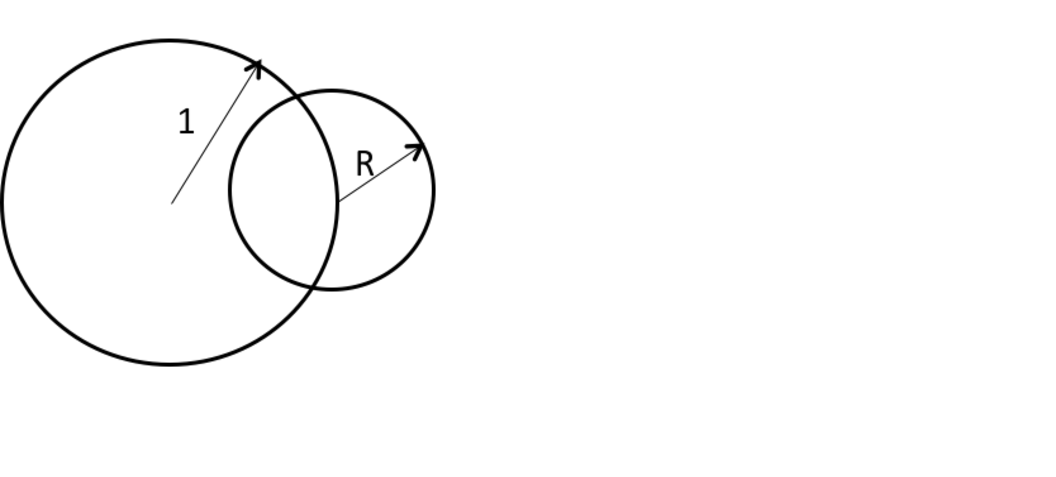
\includegraphics[width=\linewidth]{Snowman}
        \caption{Construction of Snowman molecules}
        \label{fig:snowman}
    \end{subfigure}
    \begin{subfigure}{0.5\textwidth}
        \centering
        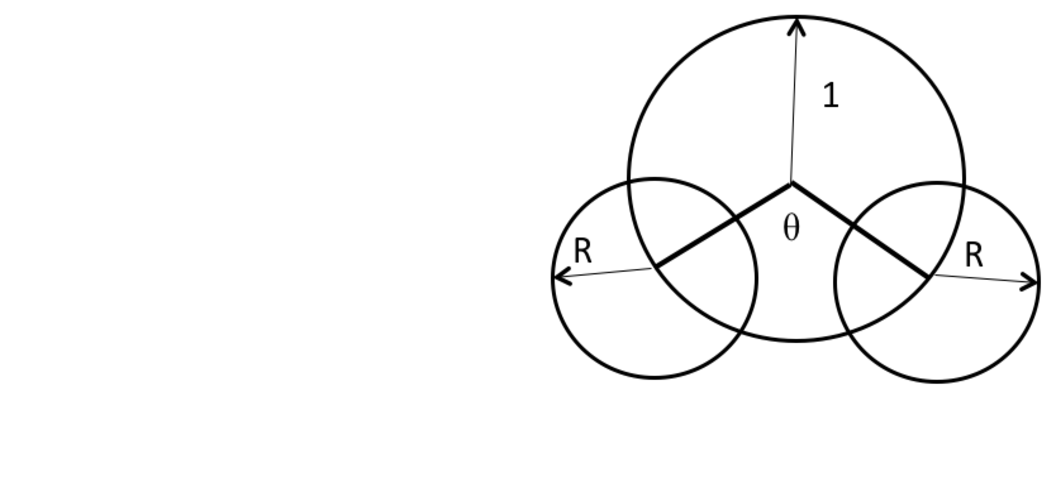
\includegraphics[width=\linewidth]{Trimer}
        \caption{Construction of Trimer molecules}
        \label{fig:trimer}
    \end{subfigure}
    \caption{Construction of the molecules used in this thesis}
    \label{fig:construction}
\end{figure}

The modified Lennard Jones potential is a potential commonly used in molecular dynamics systems due to its simplicity to calculate. It is also the potential used by most studies on glass forming binary mixtures~\tocite. The Lennard-Jones potential takes the form
\begin{equation}
    V_{LJ}(r) = 4\epsilon\left [ \left (\frac{\sigma}{r}\right )^{12} -\left ( \frac{\sigma}{r} \right )^6 \right]
\end{equation}
where $r$ is the separation of two centers and, $\epsilon$ and $\sigma$ are parameters describing the strength and the size of the potential respectively. The computational simplicity comes from the ease of computing a 6th power function, the 12th power term is then just the square of the 6th power term. In the default form the Lennard-Jones potential acts over all space, a particle would have interaction with all other particles despite most of these interactions being negligible. To reduce the number of interactions to compute the potential is commonly modified to have a cutoff distance at some small value of the potential; we chose a cutoff distance of $2.5\sigma$. The final modification to the potential is to retain the continuity of the original function, subtracting the value at the cutoff giving a function of the form
\begin{equation}
    V_{mod}(r) = \begin{cases}
        \quad V_{LJ}(r) - V_{LJ}(2.5\sigma) & \text{if } r < 2.5\sigma \\
        \quad 0  &\text{if } r >= 2.5\sigma
    \end{cases}
\end{equation}


\section{Molecular Dynamics}

The simulations in this thesis are performed using molecular dynamics, the positions of molecules are stepped through time by solving Newton's equations at each step. The software used to perform the molecular dynamics simulations is Lammps~\tocite, an open source program designed to efficiently perform large scale molecular dynamics simulations. An integral part of the optimisation achieved by Lammps is the spatial decomposition of particles amongst the available processors, allowing for efficient use use of a large number of processors~\tocite. Spatial decomposition is a technique that divides the simulation area into a grid equal to the number of processors. Each processor is then assigned an area of the grid for which it is responsible for computing. The processors are also assigned a set of \emph{ghost particles}, particles which are outside of the region the processor is responsible for computing but are close enough to be applying a force to particles in that region. The use of ghost atoms reduces the amount of communication between processors, at each step the only communication required is the updated positions of the ghost atoms. The reduction in communication is important for efficiency as it is the major speed bottleneck in alternative methods.

In a simple system like a Lennard-Jones system the standard units for various properties are cumbersome and not well matched to the specific system. Instead Lammps uses a set of reduced units, with mass $m = 1$ as the fundamental unit. A series of further units can be derived using the parameters of the Lennard-Jones potential $\sigma$ and $\epsilon$. 

\begin{table}
    \centering
    \begin{alignat*}{2}
        &\text{Mass} & m &= 1 \\
        &\text{Energy} & E^* &= E/\epsilon \\
        &\text{Temperature  }\quad& T^* &= T_k/\epsilon \\
        &\text{Length} & L^* &= L/\sigma \\
        &\text{Pressure} & P^* &= P\sigma^3/\epsilon \\
        &\text{Time} & t^* &= t\sqrt{\epsilon/(m\sigma^2)}
    \end{alignat*}
    \caption{Reduced LJ Units}
    \label{tab:reduced units}
\end{table}


The thermodynamic ensemble for the simulation is the NPT ensemble, with a constant number of particles (N), constant pressure (P) and constant temperature (T). The constant number of particles is achieved by not adding or removing any particles from the simulation, the pressure and temperature are kept constant by a Noose-Hoover thermostat\tocheck.
\towrite{Thermostat and barostat}

\section{Simulation Parameters}

\subsection{Dynamics}

The initial configuration for the dynamics runs is a grid of molecules each with a random orientation. The distance between molecules is larger than the dimensions of the molecules such that they do not contact each other. From this initial configuration the molecules are compressed into a liquid and equilibrated at a temperature $T=5$, well above the melting point. The configuration is then cooled through a series of temperatures, equilibrating at each temperature for at least the relaxation time at that temperature. The production runs at each temperature use the equilibrated configurations as a starting point to ensure the dynamics are consistent across the simulation.

\subsection{Crystal Structures}

To generate the crystal packings the isopointal algorithm developed by Toby Hudson~\tocite was used to estimate the lowest energy structures using the approximation that the lowest energy Lennard-Jones structure is the best packed hard disc structure. Large systems of the best packed structures were then generated by replicating the unit cell. These systems were then equilibrated at low temperature using the Rahman-Parinello algorithm, which allows for both the size of the simulation and the tilt of the simulation to be adjusted to lower the energy of the system. These equilibrated systems were then subjected to conjugate gradient minimisation for comparison with the amorphous packings.

For these simulations we start with the lowest energy crystals formed in the previous sections. These square regions of crystal are then duplicated in either the $x$ or the $y$ directions. The long edge of these is then divided up into two halves, with one half heated above the melting point forming a liquid, and the other half held in position. This generates an liquid/crystal interface on the two different faces of the crystal from which it is expected that crystals will grow.

These boundaries then held at a series of temperatures close to the melting point to observe the phase changes that are taking place at the boundary.

